\documentclass[11pt]{amsart}
\usepackage[T1]{fontenc}
\usepackage{lmodern,amsmath,amssymb,amsthm,microtype,booktabs,tikz}
\usepackage[margin=1.06in]{geometry}
\usepackage[hidelinks]{hyperref}
\emergencystretch=2em
\numberwithin{equation}{section}
\newtheorem{proposition}{Proposition}[section]
\newtheorem{lemma}[proposition]{Lemma}
\newcommand{\R}{\mathbb R}
\newcommand{\norm}[1]{\lVert#1\rVert}
\DeclareMathOperator{\conv}{conv}
\DeclareMathOperator{\tr}{tr}
\DeclareMathOperator{\vol}{vol}
\title[Companion notes to Foundations I]{General Theta Foundations I:\\Companion Notes to the Complete Mathematical Supplement}
\author{Qian Qi}
\date{27 September 2026}
\begin{document}
\maketitle
The separately compiled complete supplement reproduces all the preceding mathematical source files and their loaded proofs. These notes provide local refinements and an additional intrinsic conditioning statement. The main article, \emph{Sharp Noise Thresholds for Stochastic Realizations of Compact Group Experiments}, is independently complete. References to named results in the retained supplement refer to its unchanged numbering; labels are recorded in the accompanying source manifest.

\section{Finite orbits, moving representations, and the interface}
Let $H$ be a compact matrix group, $K=H^\circ$, and $G$ a dense subgroup of $H$. Let $V$ be a finite-dimensional orthogonal representation.
\begin{proposition}\label{note:fixed53}
The finite-orbit subspace $F=\{v\in V:Gv\text{ is finite}\}$ is exactly the $K$-fixed subspace. It and its orthogonal complement $E$ are $H$-invariant. For every $h\in H$, their orthogonal projections commute with $h$.
\end{proposition}
\begin{proof}
If $Gv$ is finite, it is closed, so $Hv=\overline{Gv}=Gv$. The connected set $Kv$ is finite and therefore a singleton. Conversely, if $Kv=\{v\}$, then $Hv$ has at most $|H/K|$ points. Normality of $K$ implies $H$-invariance of its fixed space. Orthogonality gives invariance of the complement; decomposing any vector into these two invariant summands proves $P_Eh=hP_E$ and $P_Fh=hP_F$.
\end{proof}
This identifies the finite-orbit reduction in the retained noisy theorem with the identity-component reduction in the new classification. The moving tensor representation in the main article is usually larger than the original moving physical space. Its dimension, and the block length, defect, and logarithmic contraction rate, depend on the chosen degree, action, and width. They do not depend on the horizon or on a positive lower bound for hidden-state masses.

The retained coordinate argument allows the action-dependent interval
\[
 \varepsilon<\frac{\rho s_*}{2\sqrt D},\qquad
 s_*=\max_i\norm{P_Ee_i},
\]
with $s_*\ge\sqrt{\dim E/D}\ge D^{-1/2}$. The interval $\varepsilon<\rho/(2D)$ is only its dimension-uniform consequence. Neither interval is claimed to be the sharp boundary. For the circle, the main article proves the larger exact boundary $\rho/2$.

Combining coordinate decoder columns into a vector is only a proof device; no joint query output is required. Likewise, the polynomial weights used in the new proof are functions of the externally supplied command word. They do not add higher-order measurements to the allowed query interface. One fixed seed and one fixed query witness the subcritical obstruction. The distinction is important for genuinely partial interfaces.

A positive word uses only actual command letters. A common-length word law is obtained by executable identity padding, not by adjoining inverse commands. The identity letter is permitted to have a nonidentity hidden-state update. Occupation counts exclude cut zero, as explicitly stated in both noisy occupation theorems. A finite net for Haar approximation uses a radius strictly smaller than one half of the positive integral gap. The gap and the approximation radius are distinct constants.

\section{Trace, support, and the one-surplus coefficient}
For a full-dimensional convex body $P$ containing zero in its interior, the support function $h_P(u)=\max_{x\in P}\langle u,x\rangle$ is strictly positive on the unit sphere, and
\begin{equation}\label{note:support53}
 \min\{\lambda\ge1:-P\subset\lambda P\}
       =\max_{\norm u=1}\frac{h_P(-u)}{h_P(u)}.
\end{equation}
Indeed containment of compact convex sets is equivalent to the corresponding support inequalities. The maximum is at least one, by exchanging $u$ and $-u$.

\begin{lemma}[Trace refinement]\label{note:trace53}
If $P\subset\R^D$ has at most $k$ vertices or at most $k$ facets, where $D+1\le k<2D$, then its origin asymmetry in \eqref{note:support53} is at least $D/(k-D)$.
\end{lemma}
\begin{proof}
Suppose first that $P$ has $m\le k$ vertices, arranged as rows of $Z$. If $-P\subset\lambda P$, convex representations of $-Z_i/\lambda$ give a nonnegative row-stochastic matrix $T$ with $T\mathbf1=\mathbf1$ and $TZ=-\lambda^{-1}Z$. The columns of $[\mathbf1,Z]$ are independent, so $1$ is an eigenvalue and $-\lambda^{-1}$ has geometric, hence algebraic, multiplicity at least $D$. Every eigenvalue has modulus at most one. Because $T$ is real, nonreal eigenvalues occur in conjugate pairs; the sum of the real parts of the remaining $m-D-1$ eigenvalues is at most $m-D-1$. Nonnegativity of the diagonal gives
\[
              0\le\tr T\le m-D-D/\lambda.
\]
Thus $\lambda\ge D/(m-D)\ge D/(k-D)$. Apply the same argument to the polar body for the facet case. Polarity shows that $P$ and its polar have the same origin asymmetry.
\end{proof}

Here is the support-cone geometry behind the retained volume increment. Suppose $rB^D\subset P\subset[-1,1]^D$, choose a unit $u$, and let $h=h_P(u)\ge r$. If $x\in-P$ has $t=\langle u,x\rangle\ge Lh$ with $L>1$, the cone from $x$ to the central radius-$r$ disk in $u^\perp$ lies in $\conv(P\cup(-P))$. Its portion above height $h$ lies outside $P$.
\begin{center}
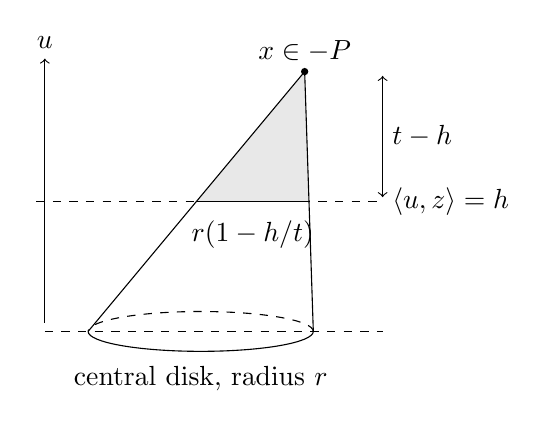
\begin{tikzpicture}[scale=1.1]
\fill[gray!18] (1.2,3)--(-.05,1.5)--(1.25,1.5)--cycle;
\draw (-1.3,0) arc[start angle=180,end angle=360,x radius=1.3,y radius=.23];
\draw[dashed] (1.3,0) arc[start angle=0,end angle=180,x radius=1.3,y radius=.23];
\draw (-1.3,0)--(1.2,3)--(1.3,0);
\draw[dashed] (-1.9,1.5)--(2.1,1.5) node[right] {$\langle u,z\rangle=h$};
\draw (-.05,1.5)--(1.25,1.5);
\draw[dashed] (-1.8,0)--(2.1,0);
\draw[->] (-1.8,.1)--(-1.8,3.15) node[above] {$u$};
\draw[<->] (2.1,1.55)--(2.1,2.95) node[midway,right] {$t-h$};
\fill (1.2,3) circle (1.2pt) node[above] {$x\in-P$};
\node at (0,-.55) {central disk, radius $r$};
\node at (.6,1.12) {$r(1-h/t)$};
\end{tikzpicture}
\end{center}
The drawing is schematic. The cross-section at height $h$ is a translated disk of radius $r(1-h/t)$, and the perpendicular height of the added cone is $t-h$. Obliqueness changes neither quantity. With $\omega_{D-1}$ the unit-ball volume in dimension $D-1$, its volume is
\[
 \frac{\omega_{D-1}}D\,r^{D-1}(1-h/t)^{D-1}(t-h)
 \ge\frac{\omega_{D-1}}D\,r^D(1-L^{-1})^{D-1}(L-1).
\]
The support plane itself has zero $D$-dimensional volume, so the use of an open region above it has no effect on the estimate. Dividing by $\vol(P)\le2^D$, and substituting $r=\rho/\sqrt D$, $L=D/2$, yields exactly
\[
 \beta_D(\rho)\ge1+
 \frac{\omega_{D-1}(D-2)^D}{2^{D+1}D^{3D/2}}\rho^D\qquad(D\ge3).
\]
In dimension three the coefficient is $\pi/(1296\sqrt3)$. The simpler $1/1024$ is a deliberately weakened rational coefficient, not an equality for the optimum.

\subsection{Exact verification of the illustrative horizon}
For $\rho=1/10$, let $x=1/1{,}024{,}000$ and $N_0=9{,}216{,}009=9(1{,}024{,}001)$. Then
\[
 N_0\log(1+x)\ge N_0\frac{x}{1+x}=9.
\]
The finite rational inequality $\sum_{j=0}^{20}9^j/j!>6000$ proves $e^9>6000=6\rho^{-3}$. Therefore $(1+\rho^3/1024)^{N_0}>6\rho^{-3}$, as required by the exact six-state theorem. The retained exact checker verifies this rational inequality. This is a sufficient horizon, not the first transition horizon. The unconditional noise-search theorem proves termination of a finite algebraic search; that search has not been executed at this illustrative horizon. No numerical positive noisy margin at that horizon is claimed in this revision.

\section{Intrinsic reachable-basis conditioning}
Fix one cut and list its finite set of actual reachable probability rows. Their span has dimension $r$. A reachable basis $B$ is an $r$-by-$k$ matrix consisting of independent rows from this list, and
\[
 P=\operatorname{rowspan}(B)\cap\Delta_{k-1},\qquad
 A(B)=\max\{\norm\alpha_1:\alpha B\in P\}.
\]
Here $\norm\alpha_1$ denotes the $\ell^1$ norm of the coefficient row. Define the basis-independent number
\begin{equation}\label{note:Amin53}
 A_{\min}=\min_{B\text{ an actual reachable basis}} A(B).
\end{equation}
\begin{proposition}\label{note:conditioning53}
The minimum in \eqref{note:Amin53} is attained, $1\le A_{\min}<\infty$, and for every supplied basis
\[
 A(B)\le\frac{\sqrt r}{\sigma_{\min}(B)}.
\]
For rational or real-algebraic supplied reachable rows, $A_{\min}$ is exactly computable by a finite collection of linear optimizations. No polynomial complexity bound or horizon-uniform upper bound follows.
\end{proposition}
\begin{proof}
There are finitely many subsets of the finite reachable-row list, and at least one is a basis. For a fixed basis the inverse coefficient map is
\[
                  \alpha=pB^T(BB^T)^{-1}.
\]
It is continuous on the compact nonempty set $P$, so $A(B)$ is finite and attained. Since every row of $B$ is itself in $P$, $A(B)\ge1$. Also $\norm p_2\le\norm p_1=1$ on the probability simplex. The least-singular-value bound gives $\norm\alpha_2\le1/\sigma_{\min}(B)$, and Cauchy--Schwarz gives the displayed inequality.

To compute $A(B)$, maximize each of the $2^r$ linear functionals $\sum_i\eta_i\alpha_i$, $\eta_i\in\{-1,1\}$, over $\alpha B\ge0$, $\alpha\mathbf1=1$. This feasible set is compact because $B$ has full row rank and its image lies in the compact simplex. Take the largest optimum, then the smallest result over the finitely many bases. Exact linear algebra and linear optimization over the supplied ordered real-algebraic field suffice. Enumerating all actual prefixes and all bases can be expensive; finiteness is not a complexity estimate.
\end{proof}
A uniform bound cannot be inferred merely from finite dimension. For the two actual rows
\[
 B=\begin{pmatrix}1&0\\1-\eta&\eta\end{pmatrix},\qquad0<\eta<1,
\]
the section is the whole probability segment. The coefficient row of $(0,1)$ is $(-(1-\eta)/\eta,1/\eta)$, of $\ell^1$ norm $(2-\eta)/\eta$. With only these two rows available there is no better basis. Thus $A_{\min}$ can diverge as $\eta\downarrow0$.

Every retained theorem stated with supplied bounds $A_t\le A$ also applies when $A_{\min,t}\le A$, by choosing a minimizing basis separately at each selected cut. This does not turn its conditioning premise into an automatic hypothesis. The new component-oscillation theorem uses neither quantity.

For separated cuts the stable-section proof applies the complete-suffix error once to each reachable basis row and then its linear extension. It does not add an independent approximation error for every internal epoch. The convention is mean error $\delta=2\varepsilon$, where $\varepsilon$ is binary total variation.

\section{Certificates and numerical resources}
The retained cubic projector criterion includes symmetry, idempotence, seed mass and range, stochastic row sums, projector-range invariance, and observable intertwining. The scalar count intentionally retains both entries of each symmetry equation, including redundant diagonal equations. It is a transparent description count, not a minimal encoding or a running-time estimate.

In the global identity
\[
 q-\lambda=\sigma_{-1}+\sum_{i=0}^n\sigma_i g_i,
\]
$\sigma_{-1}$ denotes the unweighted sum-of-squares term; it is not indexed by a missing constraint. All multipliers are sums of squares. The supplied verifier checks exact coefficient identities and positive semidefiniteness of rational Gram matrices. Principal minors give a finite criterion, but there are exponentially many of them. An exact pivoted $LDL^T$ verification with careful treatment of zero pivots can be more economical; no such replacement is credited as implemented here. Putinar positivity and the Lasserre hierarchy remain classical tools in the complete supplement, not new theorems asserted by the main article. The existing verifier accepts supplied certificates; a general discovery engine is not claimed.

In the retained rational finite-group compiler, $L$ is the bit length of the terminal Bernoulli probabilities, not a shorthand for the height of an orbit coordinate. Breadth-first orbit enumeration stores rationals in reduced form and compares them exactly. The finite-group premise ensures termination; the enumeration by itself is not a decision procedure for that premise. Probability sampling uses fewer than $2L$ expected fair bits but has no finite worst-case trial bound. The main article's free real-row model is a separate lower-bound convention and does not price arbitrary exact real arithmetic.

\end{document}
